\section{Why Use Bayesian Methods}
As discussed previously, Bayesian methods have a number powerful features: they allow analysts to  
\begin{itemize}[noitemsep]
	\item incorporate specific previous knowledge about parameters of interest;
  \item logically update knowledge about the parameter after observing sample data;
  \item make formal probability statements about parameters of interest;
	\item specify model assumptions and check model quality and sensitivity to these assumptions in a straightforward manner;
  \item provide probability distributions rather than point estimates, and 
	\item treat the data values in the sample as interchangeable. 
\end{itemize} 

\subsection{Problems and Solutions}
In particular, Bayesian methods are indicated in order to solve a number of problematic challenges in data analysis.
\begin{enumerate}
\item The dataset is small, but external related information is available: use the information in a prior. 
\item The model is extremely flexible (high-variance model) and so is prone to \textbf{overfitting}: use priors that with peaks close to 0 (this is roughly equivalent to the concept of regularization in machine learning).
\item There is an interest in determining the likelihood of parameter values, rather than just producing a ``best guess'': construct the full posterior for the parameters/variable of interest. 
\end{enumerate}
\subsection{Bayesian $A/B$ Testing}
$A/B$ testing is an excellent tool for deciding whether or not to roll out incremental features.  To perform an $A/B$ test, we divide users randomly into a test and control group, then provide the new feature to the test group while letting the control group continue to experience the current version of the product. \par If the randomization procedure is appropriate, we may be able attribute any difference in outcomes between the two groups to the changes we are rolling out without having to account for other sources of variation affecting the user behaviour. Before acting on these results, however, it is important to understand the likelihood that any observed differences is merely due to chance rather than to product modification. \par For example, it is perfectly possible to obtain different $H/T$ ratios between two fair coins if we only conduct a limited number of tosses; In the same manner, it is possible to observe a change between the $A$ and $B$ groups even if the underlying user behavior is identical.
\begin{Example} (derived from \cite{BDA_N13}) 
Wakefield Tiles is a company that sells floor tiles by mail order. They are trying to become an active player into the lucrative Chelsea market by offering a new type of tile to the region's contractors. The marketing department have conducted a pilot study and tried two different marketing methods:
\begin{itemize}[noitemsep]
	\item $A$ -- sending a colourful brochure in the mail to invite contractors to visit the company's showroom;
	\item $B$ -- sending a colourful brochure in the mail to invite contractors to visit the company's showroom, while including free tile samples.
\end{itemize}
The marketing department sent out 16 mail packages of type $A$ and 16 mail packages of type $B$. Four Chelseaites that received a package of type $A$ visited the showroom, while 8 of those receiving a package of type $B$ did the same. The company is aware that: 
\begin{itemize}[noitemsep]
\item a mailing of type $A$ costs 30\$ (includes the printing cost and postage);
\item a mailing of type $B$ costs 300\$ (additionnaly includes the cost of the free tile samples);
\item a visit to the showroom yields, on average, 1000\$ in revenue during the next year.
\end{itemize}
Which of the methods ($A$ or $B$) is most advantageous to Wakefield Tiles? \newl
\textbf{Solution:} the Bayesian solution requires the construction of a prior distribution and of a \textbf{generative model}; as part of the generative model, we will need to produce $n$ replicates of samples from the binomial distribution (which can be done in R using \texttt{rbinom(n,size,prob)}). \par The binomial distribution simulates \texttt{n} times the number of ``successes'' when performing \texttt{size} trials (mailings), where the probability of a ``success'' is \texttt{prob}.  A commonly used prior for \texttt{prob} is the uniform distribution $U(0,1)$, from which we can sample in R \textit{via} \texttt{runif(1, min = 0, max = 1)}.  
\begin{lstlisting}
# Number of replicates from the prior
n.draws <- 200000

# Prior
# This generates a probability of 
# success for mailings A and B, 
# for each of the replicates
prior <- data.frame(p.A = runif(n.draws, 0, 1), p.B = runif(n.draws, 0, 1))

# Generative model
# This tells us how many visitors to expect
# for mailing types A, B 
generative.model <- function(p.A, p.B) {
  visitors.A <- rbinom(1, 16, p.A)
  visitors.B <- rbinom(1, 16, p.B)
  c(visitors.A = visitors.A, visitors.B = visitors.B)
}

# Simulate data using the parameters 
# from the prior and the gen. model
# This generates the actual number of 
# visitors for each replicate 
sim.data <- as.data.frame( t(sapply(1:n.draws, function(i) {
  generative.model(prior$p.A[i], prior$p.B[i])})))

# Only those prior probabilities for 
# which the generative model match the 
# observed data are retained
posterior <- prior[sim.data$visitors.A == 4 & sim.data$visitors.B == 8, ] 

# Visualize the posteriors
par(mfrow = c(1,3))
hist(posterior$p.A, main = "Posterior -- probability of success with mailing A", xlab="p.A") 
hist(posterior$p.B, main = "Posterior -- probability of success with mailing B", xlab="p.B")
plot(posterior,main = "Scatterplot of probabilitie of success for mailing types A and B", xlab="p.A", ylab="p.B")
\end{lstlisting}

\newpage\noindent
The posterior distributions for the probability of success for each mailing types are shown in the figure below. 
\newl In order to estimate the average profit for each mailing type, we use the posterior distributions for the probability of success.   
\begin{lstlisting}
# Compute the estimated average profit per mailing type
avg.profit.A <- -30 + posterior$p.A * 1000 
avg.profit.B <- -300 + posterior$p.B * 1000 
hist(avg.profit.A, main = "Average Profit -- mailing A", xlab="profit.A") 
hist(avg.profit.B, main = "Average Profit -- mailing B", xlab="profit.B")
\end{lstlisting}
\noindent The expected profit is thus given by the following code:
\begin{lstlisting}
# Total expected profit
hist(avg.profit.A - avg.profit.B)
expected.avg.profit.diff <- mean(avg.profit.A - avg.profit.B)
abline(v = expected.avg.profit.diff , col = "red", lwd =2)
\end{lstlisting}
\begin{center}
  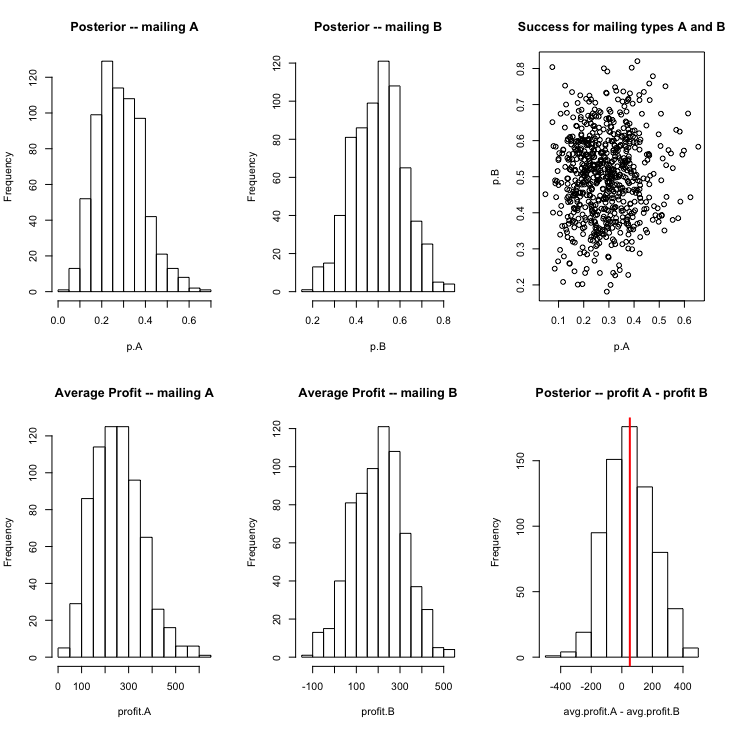
\includegraphics[width=\linewidth]{Images/example12e.png}
\end{center}
The expected profit for mailing type $A$ is around 52\$ higher than for mailing type $B$ (your numbers may vary). Keeping it simple seems to be a better idea in this context. 
\end{Example}


%----------------------------------------------------------------------------------------
% Summary
%----------------------------------------------------------------------------------------
